\documentclass[10pt,twocolumn]{article}

\usepackage[margin=0.75in]{geometry}
\usepackage{times}
\usepackage{graphicx}
\usepackage{booktabs}
\usepackage{array}
\usepackage{url}
\usepackage{xspace}
\usepackage{amsmath,amssymb}
\usepackage{cite}
\usepackage{tabularx}
\usepackage{adjustbox}
\usepackage{makecell}
\usepackage{dblfloatfix}
\usepackage{stfloats}
\usepackage{float}
\usepackage{caption}
\usepackage{placeins}


\newcommand{\tw}{TalkWeaver\xspace}
\newcommand{\repo}[1]{\texttt{\detokenize{#1}}}
\newcommand{\metric}[1]{\textsc{#1}}

\title{\tw: Evidence-Grounded Conversation Maps for Chaotic Multi-Speaker Meetings}
\author{Fu Yiyang, Liang Yurui, Lu Chenxi, Wang Yidan, Li Han, Chen Yifei}
\date{}

\begin{document}
\maketitle

\begin{abstract}
Multi-speaker meetings expose a fundamental weakness of conventional transcription pipelines: they collapse uncertain ASR, diarization, overlap, and post-processing decisions into a single fluent transcript that is difficult to verify. This design becomes particularly brittle when speech overlap, interrupted turns, ambiguous speaker boundaries, low-energy speech, and domain terminology co-occur, while unconstrained LLM correction can further obscure rather than resolve these errors. We present \textbf{TalkWeaver}, an evidence-grounded conversation-map framework that transforms fragmented post-ASR signals into a traceable record linking each utterance and proposed correction to speaker-time anchors, overlap status, retrieved domain evidence, and an explicit audit trail. By coupling speaker- and overlap-aware evidence extraction with conservative retrieval-augmented term recovery, TalkWeaver replaces opaque transcript rewriting with evidence-conditioned post-ASR processing. Experiments across FLEURS, AMI, AISHELL-4, and Earnings-22 reveal a pronounced read-speech-to-meeting robustness gap; moreover, TalkWeaver improves base-model term recall on a blind Earnings-22 subset without changing WER, while controlled overlap-safety tests show that evidence-aware correction reduces unsafe edits.
\end{abstract}

\section{Introduction}

Meetings are a primary medium for collaborative decision-making, yet their records remain difficult to trust when they are generated automatically. In realistic multi-speaker settings, a usable transcript must preserve more than lexical content: it must reveal who spoke, when they spoke, where speakers overlapped, which words were uncertain, and whether subsequent corrections remain supported by observable evidence. This requirement is particularly consequential for technical meetings, where a single mistranscribed term, misattributed utterance, or unsupported post-processing edit can distort downstream summaries, action items, and decisions.

However, contemporary meeting-transcription pipelines typically collapse heterogeneous uncertainties into a single fluent text output. Automatic speech recognition (ASR), speaker diarization, overlap detection, retrieval, and language-model post-processing are often optimized as loosely coupled stages, while the final transcript obscures the provenance of their intermediate decisions. This design is suboptimal for chaotic meetings: a transcription may appear coherent even when its speaker labels are unreliable, its overlap regions are unresolved, or its corrected terminology is weakly supported. Large language models intensify this problem. Although they can improve readability and recover domain-specific terminology, unconstrained post-processing can introduce fluent but unsupported edits that are difficult for users to inspect or reverse.

We identify two challenges that make auditable meeting transcription fundamentally different from conventional ASR post-processing. \textbf{Challenge 1: uncertainty collapse.} Multi-speaker meetings contain overlapping turns, ambiguous speaker boundaries, low-energy speech, and intermittent recognition failures. Existing pipelines frequently expose only their final transcript, thereby discarding the temporal, speaker-level, and acoustic context required to determine whether a statement should be trusted. \textbf{Challenge 2: unsupported correction.} Retrieval-augmented or LLM-based correction can recover specialized terminology, but aggressive correction policies may overwrite already correct text or hallucinate plausible alternatives. A reliable system must therefore distinguish evidence-supported recovery from speculative rewriting rather than treating every fluent revision as an improvement.

We propose \textbf{TalkWeaver}, an evidence-grounded conversation-map framework for auditable multi-speaker meeting processing. TalkWeaver represents each transcript segment as a temporal anchor that links raw ASR text, speaker attribution, timestamps, overlap status, retrieved domain terms, corrected text, and correction-audit metadata. This representation turns transcript post-processing from an opaque rewriting procedure into an evidence-conditioned decision process. Instead of hiding uncertainty, TalkWeaver carries uncertainty forward: overlap-sensitive segments remain explicitly marked, speaker-time evidence remains inspectable, and every proposed correction retains its raw source text and supporting retrieval context.

TalkWeaver directly addresses the two challenges through three coupled mechanisms. First, its temporal-anchor conversation map preserves the alignment between lexical content, speaker identity, timing, and overlap evidence, enabling downstream consumers to inspect the origin of each claim. Second, its conservative retrieval-augmented term-recovery module restricts retrieval to domain terminology and applies evidence-conditioned correction rather than unrestricted rewriting. Third, its correction audit records whether a modification was applied, rejected, or flagged for review, thereby exposing the provenance and limitations of automated post-ASR decisions. The resulting framework does not assume that all errors can be corrected automatically; rather, it prioritizes traceability when ambiguity cannot be resolved reliably.

We evaluate TalkWeaver on public subsets of FLEURS \cite{conneau2022fleurs}, AMI \cite{carletta2005ami}, AISHELL-4 \cite{fu2021aishell4}, and Earnings-22 \cite{delrio2022earnings22}, together with controlled safety analyses designed to isolate overlap-sensitive correction behavior. The evaluation covers English, French, and Mandarin, and includes a local-inference accuracy--runtime analysis in addition to the meeting-processing study. Our results reveal a pronounced gap between read speech and meeting speech; the diarization analyses further show that speaker attribution and overlap remain unresolved bottlenecks, particularly in Mandarin meeting audio. For domain-term recovery, an earlier retrieval policy improved weak ASR outputs but could degrade stronger transcripts, whereas the conservative RAG v3 policy improves base-model term recall on a blind Earnings-22 subset without changing WER. Controlled overlap-safety experiments further support the need for evidence-aware correction, while our independent EvidenceGate analyses expose the limits of relying on controlled data to claim real-world correction-decision generalization.

Our contributions are as follows:

\begin{itemize}
    \item We formulate chaotic meeting transcription as an \textit{evidence-grounded auditing problem}, rather than a transcription or summarization problem alone, and introduce a temporal-anchor conversation-map representation that preserves speaker, timing, overlap, retrieval, and correction provenance.
    \item We develop an auditable multi-stage framework that combines ASR, speaker-time alignment, overlap-aware evidence extraction, conservative domain-term retrieval, and correction auditing without collapsing intermediate uncertainty into a single opaque transcript.
    \item We provide a multilingual empirical characterization spanning English, French, and Mandarin public subsets, showing that read-speech ASR performance substantially overestimates robustness in realistic multi-speaker meetings and exposing the accuracy--runtime trade-off of local inference.
    \item We demonstrate that conservative evidence-conditioned retrieval can improve domain-term recall without degrading WER, and we provide controlled safety and leakage analyses that clarify both the promise and the current limits of automated correction decisions.
\end{itemize}

\section{Related Work}

\subsection{Multi-Speaker ASR, Diarization, and Overlap-Aware Meeting Processing}

Recent advances in multilingual ASR have substantially improved transcription quality for clean read speech, while open diarization toolkits have made it increasingly practical to estimate ``who spoke when'' in conversational recordings \cite{radford2023whisper,bredin2020pyannote}. A parallel line of work seeks to make meeting transcription more structurally faithful by integrating speaker segmentation, turn attribution, overlap modeling, and language-model reasoning. DiarizationLM demonstrates that language models can improve speaker-attributed transcripts through diarization-aware post-processing, whereas DM-ASR and TagSpeech incorporate speaker and temporal structure more directly into multi-speaker recognition \cite{wang2024diarizationlm,li2026dmasr,huo2026tagspeech}. These efforts establish an essential premise: lexical accuracy alone is insufficient when downstream use depends on speaker identity, temporal ordering, and interaction structure.

However, most pipelines still treat ASR, diarization, and overlap handling as separate prediction problems whose outputs are merged only at the end. This design obscures the dependency structure among errors. A lexical hypothesis may be plausible but originate from an overlap region; a speaker label may be assigned despite an uncertain boundary; and a temporally aligned transcript may still conceal the evidence required to assess its reliability. TalkWeaver is positioned differently: rather than optimizing a single speaker-attributed transcript, it preserves ASR hypotheses, speaker-time assignments, overlap indicators, and downstream decisions in a unified evidence-carrying representation.

\subsection{Retrieval-Augmented and LLM-Based ASR Error Correction}

Post-ASR correction increasingly uses retrieval and large language models to address errors that acoustic models struggle to resolve, particularly rare entities, domain terminology, punctuation, and contextual ambiguity. Retrieval-augmented correction can retrieve candidate entities from an external knowledge store and condition a correction model on those candidates \cite{pusateri2024retrieval}. This direction demonstrates that text-side post-processing can recover errors that remain difficult for acoustic decoding alone, especially when domain knowledge is available.

However, correction quality cannot be assessed solely by fluency or aggregate WER. Retrieved terms can trigger false-positive substitutions when they are semantically plausible but unsupported by the utterance, while LLM-based correction can rewrite already correct text or complete partial speech speculatively. TalkWeaver therefore treats retrieval as evidence to be audited rather than a license for free-form rewriting: a proposed modification remains linked to its raw ASR source, temporal anchor, overlap state, retrieved candidates, and audit outcome. This distinction is central in meeting settings, where a fluent correction can be more harmful than an explicit uncertainty label.

\subsection{Auditing, Provenance, and Uncertainty in Speech-Centric Systems}

Reliable speech systems must expose not only what they predict, but also why a user should trust the prediction. Prior analyses of speech-to-text hallucinations show that transcription systems can generate plausible content that does not faithfully reflect the source audio, creating risks for downstream decision-making \cite{koenecke2024careless}. In parallel, system designs that retain confidence signals and review mechanisms recognize that automated predictions may require human inspection in consequential settings.

A major limitation is that these principles are rarely operationalized as a shared representation spanning the full post-ASR pipeline. Confidence scores alone do not reveal whether an error arose from lexical recognition, speaker attribution, overlap, retrieval, or correction. Likewise, an audit layer added after free-form rewriting cannot reconstruct evidence that was discarded earlier in the pipeline. TalkWeaver addresses this gap through a temporal-anchor conversation map that carries heterogeneous evidence forward rather than compressing it into a single final transcript. Each segment maintains its raw text, speaker-time context, overlap status, retrieved terminology, corrected text, and correction state, enabling users and downstream components to distinguish supported recovery from unresolved ambiguity.

\subsection{Positioning of TalkWeaver}

TalkWeaver occupies a distinct point in the design space of meeting transcription systems. Unlike conventional ASR and diarization pipelines that prioritize a finalized transcript, TalkWeaver treats the transcript as an auditable artifact whose reliability depends on preserved provenance. Unlike retrieval-augmented correction systems that focus primarily on lexical recovery, it restricts retrieval to evidence-conditioned domain-term recovery and records the basis of each modification. Unlike LLM post-processing frameworks that evaluate correction as a text-generation problem, it represents correction as a traceable decision embedded within speaker-time and overlap-aware evidence. Consequently, TalkWeaver does not claim to replace state-of-the-art ASR or diarization models; it provides a framework for exposing, organizing, and auditing the uncertainty that these components inevitably leave behind in chaotic multi-speaker meetings.

\section{Methodology}
\label{sec:method}

\subsection{Problem Formulation}

We formulate chaotic meeting transcription as an \emph{evidence-grounded post-ASR processing} problem. Given a meeting recording
\[
x:[0,T]\rightarrow \mathbb{R},
\]
where \(T\) denotes the recording duration, TalkWeaver produces an auditable conversation map rather than a single finalized transcript. The map must preserve the provenance of each transcription unit and each subsequent modification.

An ASR backend converts \(x\) into timestamped lexical hypotheses:
\[
\mathcal{H}
=
f_{\mathrm{ASR}}(x)
=
\left\{
h_i=(\hat{y}_i,a_i,b_i,\kappa_i)
\right\}_{i=1}^{N},
\]
where \(\hat{y}_i\) denotes the raw ASR hypothesis for unit \(i\), \([a_i,b_i]\subseteq[0,T]\) denotes its temporal interval, and \(\kappa_i\) denotes an optional ASR confidence score when available. Depending on the ASR backend, a unit may correspond to a word, phrase, or segment.

In parallel, a diarization backend produces estimated speaker turns:
\[
\mathcal{D}
=
f_{\mathrm{DIA}}(x)
=
\left\{
d_j=(\ell_j,u_j,v_j)
\right\}_{j=1}^{M},
\]
where \(\ell_j\) is a speaker label and \([u_j,v_j]\) is the associated active interval. Let \(\mathcal{V}\) denote a provenance-aware inventory of domain terms and supporting knowledge sources. TalkWeaver maps \((\mathcal{H},\mathcal{D},\mathcal{V})\) to
\[
\mathcal{C}
=
\left\{
c_i
\right\}_{i=1}^{N}
\cup
\mathcal{E},
\]
where \(c_i\) is an evidence-carrying temporal anchor and \(\mathcal{E}\) contains optional interaction-event candidates, such as overlap or interruption candidates. Each anchor retains raw text, timing, speaker evidence, overlap state, retrieved terminology, corrected text when applicable, and correction-audit metadata. The objective is therefore not to maximize transcript fluency alone, but to preserve sufficient evidence for users and downstream systems to assess why a transcript fragment or correction should be trusted.

\subsection{Overall Framework}

Figure~\ref{fig:architecture} illustrates the TalkWeaver pipeline. The framework first preprocesses the input audio and applies ASR to obtain timestamped hypotheses. It then aligns these hypotheses with diarization turns, derives overlap-aware temporal anchors, retrieves domain terminology for uncertain expressions, and passes the resulting evidence to a constrained correction module. Finally, an audit layer records the relationship between the original hypothesis, the proposed correction, and the evidence used to justify, reject, or defer the modification.

This ordering is intentional. Conventional post-ASR pipelines often treat transcription as a fixed intermediate output and apply correction only after uncertainty from earlier stages has already been discarded. TalkWeaver instead carries this uncertainty forward before correction occurs. Consequently, a retrieved term is not treated as an unconditional replacement candidate, and a fluent revision is not treated as inherently reliable. The correction module receives evidence specifying \emph{where} the text originated, \emph{who} may have spoken it, \emph{whether} overlap affected the interval, and \emph{which} retrieved terms support a potential modification.

\begin{figure*}[t]
\centering
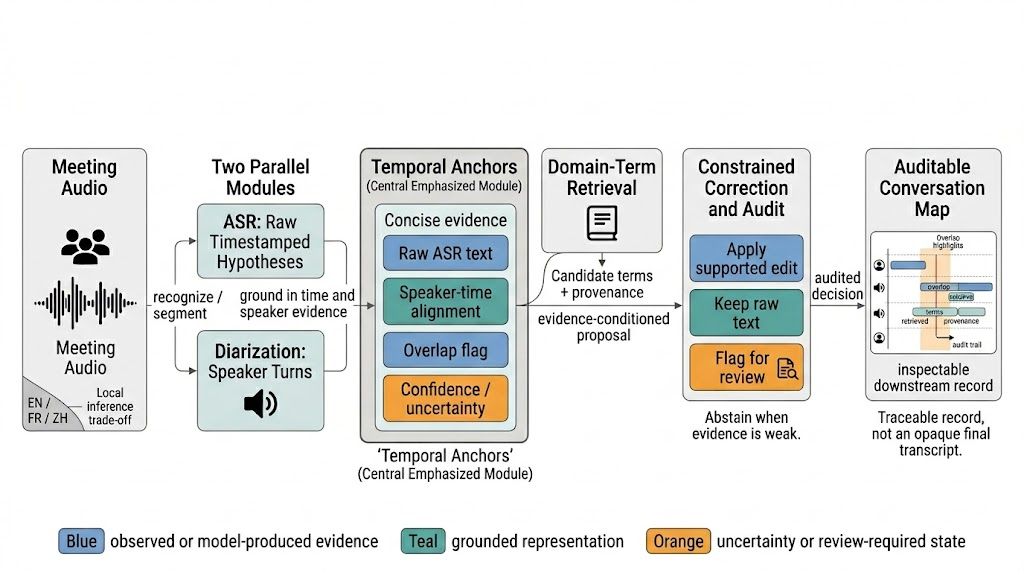
\includegraphics[width=0.92\textwidth]{figures/aec.jpg}
\caption{TalkWeaver converts heterogeneous post-ASR signals into evidence-grounded temporal anchors. Rather than directly rewriting a transcript, the framework retains speaker-time alignment, overlap status, retrieval provenance, and correction-audit outcomes in an auditable conversation map.}
\label{fig:architecture}
\end{figure*}

\subsection{Temporal-Anchor Construction}

\paragraph{Speaker-time alignment.}
For each ASR unit \(h_i\), TalkWeaver defines the temporal interval
\[
I_i=[a_i,b_i].
\]
To associate this unit with speaker evidence, we compute the temporal support for each diarized speaker label:
\[
\lambda_{\ell}(I_i)
=
\sum_{j:\ell_j=\ell}
\left|
I_i \cap [u_j,v_j]
\right|,
\]
where \(|\cdot|\) denotes interval duration. The primary speaker assignment is
\[
\hat{s}_i
=
\begin{cases}
\operatorname*{arg\,max}_{\ell}\lambda_{\ell}(I_i),
& \text{if } \max_{\ell}\lambda_{\ell}(I_i)>0,\\[4pt]
\texttt{UNKNOWN},
& \text{otherwise}.
\end{cases}
\]

TalkWeaver does not interpret \(\hat{s}_i\) as ground truth. Instead, it retains the full set of speakers with local temporal support:
\[
\mathcal{S}_i
=
\left\{
\ell
\mid
\lambda_{\ell}(I_i)>0
\right\}.
\]
This design separates the speaker label required for visualization from the ambiguity that remains in the diarization evidence. A single label may be convenient for grouping utterances, whereas \(\mathcal{S}_i\) exposes competing speaker assignments that should remain visible to later modules and users.

\paragraph{Overlap evidence.}
Let the active speaker set at time \(t\) be
\[
\mathcal{A}(t)
=
\left\{
\ell_j
\mid
u_j \leq t \leq v_j
\right\}.
\]
TalkWeaver marks unit \(i\) as overlap-affected when at least two speaker labels are active during any portion of its interval:
\[
o_i
=
\mathbb{I}
\left[
\exists t\in I_i:
\left|
\mathcal{A}(t)
\right|
\geq 2
\right].
\]

The overlap indicator does not assert that every token in the unit was jointly spoken, nor does it infer that a social interruption occurred. Instead, it provides a conservative warning that the ASR hypothesis and speaker assignment were produced under a potentially confounded acoustic condition. This distinction is important because temporal overlap is directly observable from diarization output, whereas behavioral interpretations require stronger evidence.

\paragraph{Temporal-anchor representation.}
The resulting raw temporal anchor is represented as
\[
c_i^{\mathrm{raw}}
=
\left(
\hat{y}_i,
I_i,
\hat{s}_i,
\mathcal{S}_i,
o_i,
\kappa_i
\right).
\]
This representation forms the core unit of TalkWeaver. Rather than collapsing lexical content, speaker identity, and overlap status into a single unqualified sentence, it retains the uncertainty surrounding the generation of each transcript fragment. Subsequent retrieval, correction, and review modules therefore operate on evidence-bearing anchors rather than decontextualized text.

\subsection{Evidence-Conditioned Domain-Term Recovery}

Meeting recordings often contain abbreviations, named entities, technical terminology, and project-specific vocabulary that acoustic models misrecognize. TalkWeaver therefore uses retrieval as targeted lexical evidence rather than as a generic mechanism for unrestricted generation. Let
\[
\mathcal{V}
=
\bigcup_{p\in\mathcal{P}}
\mathcal{V}_p
\]
denote a partitioned knowledge inventory, where each partition \(\mathcal{V}_p\) corresponds to a provenance-aware source, such as domain terminology, ASR terminology, speaker-related metadata, or project documentation. For term recovery, TalkWeaver restricts retrieval to the domain-term partition.

Given a normalized query \(q_i\) derived from \(\hat{y}_i\), the retriever returns the top-\(K\) candidate terms:
\[
R_i
=
\operatorname{TopK}_{v\in\mathcal{V}_{\mathrm{term}}}
\phi(q_i,v),
\]
where \(\phi\) denotes the configured similarity function. Each element in \(R_i\) includes both a candidate term and its source provenance.

The central intuition is that retrieval should constrain correction rather than authorize it. A retrieved term may be lexically similar to an ASR error while still being unsupported by the utterance or inappropriate in context. Accordingly, TalkWeaver attaches \(R_i\) to the temporal anchor as evidence instead of directly replacing \(\hat{y}_i\). This conservative design mitigates a common failure mode of retrieval-augmented correction: a plausible external term may improve a weak ASR hypothesis while degrading an already accurate transcript.

\subsection{Constrained Correction and Audit Provenance}

For each temporal anchor, TalkWeaver constructs an evidence bundle
\[
e_i
=
\left(
c_i^{\mathrm{raw}},
R_i
\right),
\]
which contains the raw ASR text, interval, speaker evidence, overlap state, optional confidence, and retrieved terminology. A configured correction operator \(\Gamma\), implemented through rule-based or LLM-assisted post-processing, receives this bundle and produces a proposed output:
\[
\tilde{y}_i
=
\Gamma(\hat{y}_i,e_i).
\]

Crucially, \(\tilde{y}_i\) is a proposal rather than an unconditional replacement. The framework explicitly permits the no-change outcome:
\[
\tilde{y}_i=\hat{y}_i,
\]
which is essential when evidence is weak, overlap is substantial, or retrieved candidates do not justify a modification.

TalkWeaver then computes an edit record:
\[
\Delta_i
=
\operatorname{Diff}
\left(
\hat{y}_i,\tilde{y}_i
\right),
\]
and associates it with an audit object:
\[
a_i
=
\left(
\Delta_i,
R_i,
I_i,
\mathcal{S}_i,
o_i,
\eta_i
\right),
\]
where \(\eta_i\) denotes the audit outcome, including an applied modification, rejected proposal, unchanged hypothesis, or review-required case. Although the exact policy may vary across correction backends, the framework always records the raw text, candidate revision, and evidence available at decision time.

This audit layer addresses a structural weakness of unconstrained transcript rewriting. Once a language model produces a polished sentence, a user cannot reliably determine whether an edit originated from acoustic evidence, a diarization artifact, retrieved external knowledge, or the language model's prior. TalkWeaver preserves these distinctions explicitly. A corrected term remains traceable to its temporal anchor and retrieved evidence, while overlap-sensitive or speaker-ambiguous anchors can remain unresolved instead of being silently normalized into fluent but weakly supported text.

\subsection{Conversation Map Output}

The final conversation map contains audited anchors and optional interaction-event candidates:
\[
\mathcal{C}
=
\left\{
\left(
c_i^{\mathrm{raw}},
R_i,
\tilde{y}_i,
a_i
\right)
\right\}_{i=1}^{N}
\cup
\mathcal{E}.
\]
The map supports multiple downstream views without changing the underlying evidence. For example, a speaker timeline groups anchors according to \(\hat{s}_i\), an overlap view filters anchors with \(o_i=1\), and a correction view displays \(\Delta_i\) together with \(R_i\) and \(\eta_i\). Because each view references the same evidence-bearing objects, TalkWeaver avoids generating independent summaries or visualizations that may drift from the original transcript provenance.

\subsection{Optimization and Training Strategy}

TalkWeaver does not introduce a new end-to-end trainable model or optimize a task-specific composite loss. Instead, it composes pretrained ASR and diarization backends with inference-time alignment, retrieval, constrained correction, and audit modules. The parameters of the ASR and diarization backends remain fixed during the main pipeline evaluation, while retrieval and audit components operate through deterministic or configured inference policies.

Accordingly, we evaluate TalkWeaver through task-specific metrics rather than a unified training objective. These metrics include ASR error rates, diarization error rate, overlap-related measures, domain-term recall and precision, correction-audit statistics, and controlled safety outcomes. We analyze a learned EvidenceGate separately in controlled experiments; it is not treated as the central TalkWeaver model or as evidence of end-to-end real-world generalization. This separation is deliberate: the evaluation measures whether evidence-grounded representation and conservative post-ASR processing improve traceability and targeted term recovery, while explicitly reporting the limitations of learned correction-decision policies trained on controlled data.


\section{Experiments}
\label{sec:experiments}

\subsection{Experimental Setup}

\paragraph{Evaluation protocol.}
We evaluate TalkWeaver as an evidence-grounded post-ASR framework rather than as a replacement for the ASR or diarization backends. Accordingly, we separate \emph{real public audio}, \emph{controlled text fixtures}, and \emph{proxy measurements}. The main paper reports real-audio results for ASR, diarization, automatic map construction, and domain-term recovery; it reports controlled experiments only when analyzing correction safety and leakage. We do not use mock/demo outputs or local runtime proxies to support accuracy or deployment claims.

Table~\ref{tab:exp_data} summarizes the evaluation sources. The real-audio subsets draw from FLEURS \cite{conneau2022fleurs}, the AMI Meeting Corpus \cite{carletta2005ami}, AISHELL-4 \cite{fu2021aishell4}, and Earnings-22 \cite{delrio2022earnings22}. The public subsets are intentionally modest and should not be interpreted as full-corpus benchmarks. They provide a reproducible contrast between read speech and multi-speaker meeting speech, a real-audio testbed for domain-term recovery, and held-out meeting subsets for automatic evidence-map construction.

\begin{table*}[t]
\centering
\scriptsize
\begin{tabular}{p{0.19\textwidth}p{0.12\textwidth}p{0.13\textwidth}p{0.11\textwidth}p{0.33\textwidth}}
\toprule
Source & Evidence type & Evaluation size & Language & Role in this study \\
\midrule
FLEURS formal subset & Real public audio & 30 clips within a 50-clip manifest & en/fr/zh-CN & Read-speech ASR reference condition \\
AMI formal and held-out subsets & Real public audio & 8 formal clips; 24 held-out clips & en & Meeting ASR, diarization, and automatic map construction \\
AISHELL-4 60x20 subset & Held-out real audio & 60 clips; 29 clips with usable diarization/map outputs & zh-CN & Mandarin meeting ASR, diarization, and automatic map construction \\
Earnings-22 v2/v3 subsets & Held-out real audio & 12 files in v2; 6 files in frozen v3 & en & Domain-term retrieval and conservative correction \\
whisper.cpp Level 1 & Local-machine proxy & 76 rows & en/fr/zh-CN & Local-inference accuracy--runtime trade-off; not phone-device deployment \\
Term and overlap fixtures & Controlled text & 175 term rows; 80 overlap rows & en/fr/zh-CN & Mechanism and safety stress tests \\
EvidenceGate held-out set & Controlled authored proposals & 90 proposals & multilingual & Leakage and generalization audit \\
\bottomrule
\end{tabular}
\caption{Evaluation sources and evidence boundaries. Exact repository paths and additional artifacts are recorded in the claim audit. None of the public subsets is presented as a full-corpus benchmark.}
\label{tab:exp_data}
\end{table*}

\paragraph{Backends, baselines, and metrics.}
For the real-audio pipeline, we use fixed ASR and diarization backends and evaluate their outputs before and after evidence-grounded post-ASR processing. RQ1 reports word error rate (WER), character error rate (CER), diarization error rate (DER), Jaccard error rate (JER), overlap F1, and real-time factor (RTF). RQ2 measures whether the automatic workflow produces the expected evidence-bearing objects: temporal anchors, speaker-labeled anchors, overlap anchors, interaction-event candidates, and review flags. RQ3 compares ASR-only transcripts with conservative retrieval variants using WER, domain-term recall, and domain-term F1. RQ4 evaluates controlled correction behavior using safety pass rate, forbidden-change counts, macro F1, review recall, and unsafe-accept rate. We retain raw ASR outputs throughout evaluation and do not regard fluent rewriting alone as a success criterion.

\subsection{RQ1: How Much Harder Is Meeting Speech Than Read Speech?}
\label{sec:rq1}

\paragraph{Finding.}
Meeting speech produces a pronounced degradation in both lexical recognition and speaker-related evidence. Figure~\ref{fig:asr_error} and Table~\ref{tab:rq1} show that the FLEURS Mandarin read-speech subset is substantially easier than the available AISHELL-4 Mandarin meeting subsets. With the base ASR backend, CER increases from \(0.113\) on FLEURS zh-CN to \(0.610\) on the 12-clip AISHELL-4 formal sanity subset and \(0.537\) on the broader 60-clip subset. The small model reduces AISHELL-4 CER to \(0.482\), but approximately doubles RTF relative to the base model.

English meeting speech exhibits the same pattern. Base-model WER reaches \(0.398\) on the AMI formal subset and \(0.349\) on the held-out AMI subset; the small model improves the latter to \(0.299\) at a higher RTF. These comparisons are not claims about corpus-level ranking because the subsets differ in language, recording condition, and composition. Instead, they establish the operational condition that motivates TalkWeaver: performance measured on clean read speech can substantially overestimate robustness in multi-speaker meetings.

\begin{figure}[t]
\centering
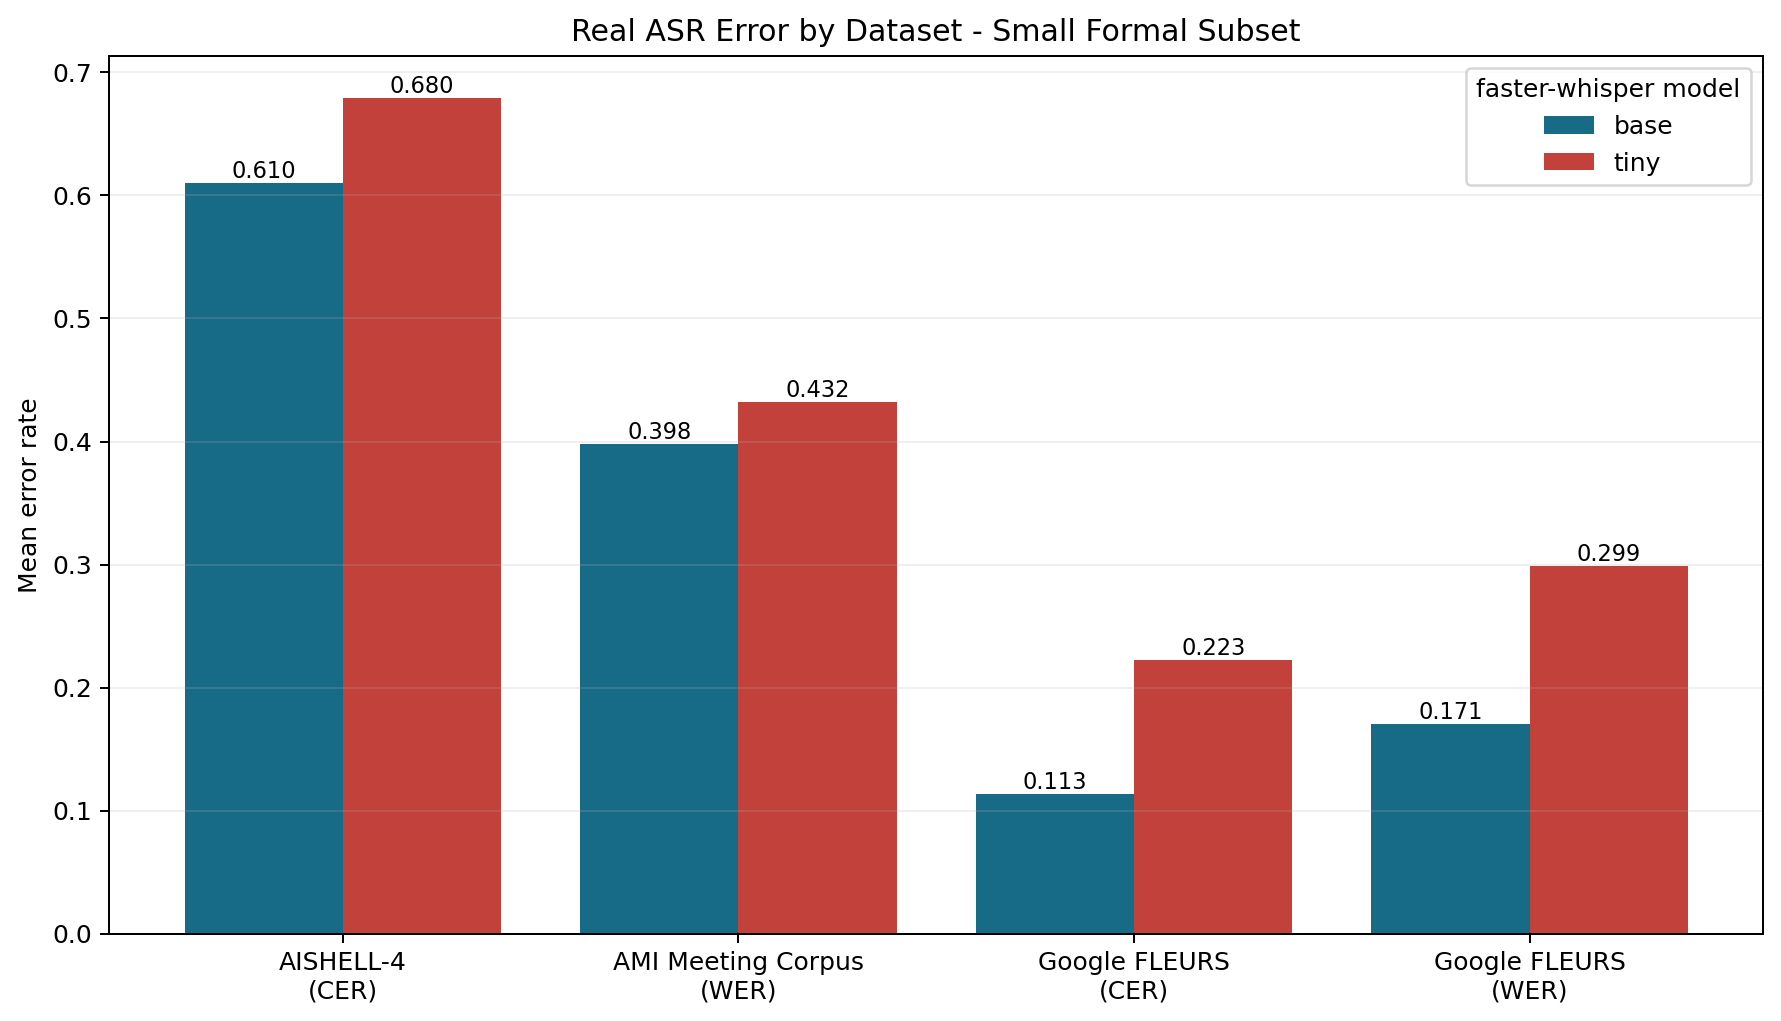
\includegraphics[width=\columnwidth]{figures/asr_error_by_dataset.png}
\caption{ASR error across the evaluated public subsets. The contrast characterizes the read-speech-to-meeting gap in the available data; it is not a full-corpus benchmark.}
\label{fig:asr_error}
\end{figure}

\begin{table*}[t]
\centering
\scriptsize
\begin{tabular}{llrrrrr}
\toprule
\multicolumn{7}{c}{\textbf{ASR}} \\
\midrule
Dataset & Model & Clips & Metric & Error & RTF & Evaluation role \\
\midrule
FLEURS en & base & 10 & WER & 0.114 & 0.085 & Multilingual read-speech coverage \\
FLEURS fr & base & 10 & WER & 0.227 & 0.078 & Multilingual read-speech coverage \\
FLEURS zh-CN & base & 10 & CER & 0.113 & 0.061 & Multilingual read-speech reference \\
AISHELL-4 formal & base & 12 & CER & 0.610 & 0.050 & Mandarin meeting sanity subset \\
AISHELL-4 60x20 & base & 60 & CER & 0.537 & 0.071 & Mandarin meeting subset \\
AISHELL-4 60x20 & small & 60 & CER & 0.482 & 0.137 & Accuracy--runtime comparison \\
AMI formal & base & 8 & WER & 0.398 & 0.055 & English meeting sanity subset \\
AMI held-out & base & 24 & WER & 0.349 & 0.072 & English meeting subset \\
AMI held-out & small & 24 & WER & 0.299 & 0.176 & Accuracy--runtime comparison \\
\midrule
\multicolumn{7}{c}{\textbf{Diarization and overlap}} \\
\midrule
Dataset & Clips & DER & JER & Overlap F1 & RTF & Evaluation role \\
\midrule
AMI held-out & 24 & 0.106 & 0.307 & 0.490 & 0.692 & English meeting subset \\
AISHELL-4 60x20 & 29 & 0.327 & 0.713 & 0.262 & 0.505 & Mandarin meeting subset \\
\bottomrule
\end{tabular}
\caption{RQ1 results from the frozen public-subset summaries. Meeting speech degrades both lexical recognition and overlap-related speaker evidence.}
\label{tab:rq1}
\end{table*}

The diarization results reinforce this conclusion. AMI achieves a usable DER of \(0.106\), but overlap F1 remains \(0.490\). On AISHELL-4, DER rises to \(0.327\), JER to \(0.713\), and overlap F1 falls to \(0.262\). These residual errors make a finalized, unqualified transcript an inadequate representation of meeting evidence: downstream correction and visualization should retain speaker-time and overlap uncertainty rather than erase it.

\paragraph{Multilingual coverage.}
The evaluation spans English, French, and Mandarin so that TalkWeaver is not characterized as an English-only system. The FLEURS read-speech subset covers all three languages, while AMI provides English meeting speech and AISHELL-4 provides Mandarin meeting speech. With the base backend, the evaluated FLEURS subsets yield English WER \(0.114\), French WER \(0.227\), and Mandarin CER \(0.113\). In contrast, the Mandarin AISHELL-4 meeting subset remains substantially harder. Together with the automatic Mandarin conversation-map results in RQ2, these findings establish multilingual pipeline coverage on the evaluated subsets. They do not establish language-invariant performance, full cross-lingual robustness, or a multilingual benchmark ranking.

\paragraph{Local-inference trade-off.}
We additionally characterize a deployment-oriented local-inference trade-off using existing whisper.cpp measurements \cite{ggerganov2023whispercpp}. On the AMI proxy rows, the tiny model runs faster than the base model (RTF \(0.031\) versus \(0.056\)) but yields higher WER (\(0.382\) versus \(0.351\)); the same ordering holds after transcript cleaning. These results make the accuracy--runtime tension explicit for local inference, while Appendix Figure~\ref{fig:app_rtf} and Table~\ref{tab:app_mobile} provide the complete measurements. They are local-machine or mobile-style proxy results, not true phone-device measurements.

\subsection{RQ2: Can TalkWeaver Construct Auditable Conversation Maps from Real Meeting Audio?}
\label{sec:rq2}

\paragraph{Finding.}
Yes. TalkWeaver constructs temporal-anchor conversation maps end to end on both AMI and AISHELL-4 held-out meeting subsets. On AMI, the automatic workflow produces, on average per clip, \(4.75\) anchors, \(4.25\) speaker-labeled anchors, \(1.79\) overlap anchors, \(2.04\) event candidates, and \(2.29\) review flags. On AISHELL-4, the workflow produces \(6.76\) anchors, \(4.48\) speaker-labeled anchors, \(0.38\) overlap anchors, \(0.24\) event candidates, and \(2.66\) review flags per scored clip.

These counts do not measure readability, user trust, or social-interaction accuracy. They instead verify the operational claim of the framework: the system carries ASR output, diarization evidence, overlap markers, and review states into a common auditable representation rather than emitting only a final transcript. Figure~\ref{fig:workflow_completeness} visualizes the evidence objects produced by the workflow.

\begin{figure}[t]
\centering

\includegraphics[width=\columnwidth]{figures/workflow_ablation_completeness.png}
\caption{Evidence objects produced by the TalkWeaver workflow. The figure illustrates map structure and review artifacts; variants using reference-assisted inputs are not interpreted as automatic accuracy results.}
\label{fig:workflow_completeness}
\end{figure}

The interruption analysis is intentionally narrower. Manual review labeled all ten selected AMI candidate windows as interruption behavior, yielding candidate precision \(1.0\). Because the study does not include an exhaustively annotated timeline or sampled non-candidate windows, recall and F1 are unavailable. We therefore report this result as candidate-level precision only; Appendix Table~\ref{tab:app_interruption} records the protocol boundary.

\subsection{RQ3: Can Conservative Retrieval Recover Domain Terms Without Degrading Transcript Quality?}
\label{sec:rq3}

\begin{table*}[t]
\centering
\footnotesize
\setlength{\tabcolsep}{3.5pt}
\renewcommand{\arraystretch}{1.12}
\begin{adjustbox}{max width=\textwidth}
\begin{tabular}{llrrrrrr}
\toprule
Subset & Variant & Model & Files & WER & Term Recall & Term F1 & Applied / Reviewed \\
\midrule
v3 blind & ASR only & base & 6 & 0.212 & 0.833 & 0.833 & 0 / 0 \\
v3 blind & RAG EvidenceGate v3 & base & 6 & 0.212 & 1.000 & 0.833 & 2 / 1 \\
v3 blind & RAG + LLM verifier v3 & base & 6 & 0.212 & 1.000 & 0.833 & 2 / 2 \\
v3 blind & ASR only & tiny & 6 & 0.252 & 0.833 & 0.833 & 0 / 0 \\
\midrule
v2 blind & ASR only & tiny & 12 & 0.222 & 0.875 & 0.889 & 0 / 0 \\
v2 blind & RAG + LLM verifier v2 & tiny & 12 & 0.222 & 0.958 & 0.931 & 2 / 0 \\
v2 blind & ASR only & base & 12 & 0.187 & 0.958 & 0.972 & 0 / 0 \\
v2 blind & RAG + LLM verifier v2 & base & 12 & 0.187 & 0.958 & 0.931 & 1 / 4 \\
\bottomrule
\end{tabular}
\end{adjustbox}
\caption{RQ3 results on Earnings-22. Conservative v3 retrieval recovers base-model term recall without WER drift; v2 exposes the failure of indiscriminate correction on stronger ASR output.}
\label{tab:rq3}
\end{table*}

\paragraph{Finding.}
Conservative retrieval improves term recall on the frozen Earnings-22 v3 subset without changing aggregate WER, but it does not establish a general improvement in transcript quality. Table~\ref{tab:rq3} reports the full comparison. On the six-file v3 subset, base-model term recall increases from \(0.833\) to \(1.000\) for both the EvidenceGate v3 and LLM-verifier v3 variants, while WER remains \(0.212\). Term F1 remains \(0.833\), so the appropriate conclusion is targeted recall recovery without WER drift, not universal correction superiority.

The earlier v2 subset provides the counterexample that motivates conservative design. RAG improves tiny-model term F1 from \(0.889\) to \(0.931\), but reduces base-model term F1 from \(0.972\) to \(0.931\). This asymmetry shows that retrieval is useful when the underlying ASR hypothesis leaves genuine lexical room for recovery, yet can damage a stronger transcript when evidence does not justify intervention. TalkWeaver therefore treats retrieval as a constrained source of evidence rather than a general rewriting license.

Appendix Figure~\ref{fig:app_term_f1} reports the controlled term-rescue study. It isolates retrieval mechanisms on text fixtures, but does not support a public-audio generalization claim.

\subsection{RQ4: What Safety Boundaries Limit Automated Correction Decisions?}
\label{sec:rq4}

\paragraph{Finding.}
Evidence-aware correction improves safety in controlled overlap cases, but current learned correction gates do not justify deployment claims. Table~\ref{tab:rq4} separates these two conclusions. In authored high-overlap fixtures, overlap-aware rule-based and LLM-assisted variants achieve a safety pass rate of \(1.000\), whereas the rule-based variant without overlap awareness has a safety pass rate of \(0.000\) and produces three forbidden changes. This result supports the design principle that overlap should route uncertain edits toward audit or abstention. It does not constitute a real-audio correction benchmark.

\begin{table*}[t]
\centering
\footnotesize
\setlength{\tabcolsep}{4pt}
\renewcommand{\arraystretch}{1.15}
\begin{tabularx}{\textwidth}{p{0.20\textwidth}p{0.17\textwidth}X X}
\toprule
Experiment & Evidence Setting & Result & Interpretation \\
\midrule
Overlap safety fixtures &
Controlled high-overlap cases &
Overlap-aware rule and LLM variants achieve safety pass \(1.000\); the unaware rule reaches \(0.000\) and produces three forbidden changes. &
Overlap evidence should constrain correction. This is controlled-fixture evidence rather than a real-audio benchmark. \\

EvidenceGate feature audit &
Controlled audit &
The audited feature set includes pre-decision fields, risky reference-derived fields, direct label proxies, and post-decision audit fields. &
Strong audit-aware scores can be leakage-prone and cannot support predictive deployment claims. \\

Evidence-only grouped validation &
Controlled validation &
Random forest macro F1 \(0.976\); unsafe accept \(0.000\). &
Internal grouped validation remains optimistic. \\

Strict independent held-out set &
Controlled held-out authored proposals &
Best macro F1 \(0.325\); review recall \(0.033\); unsafe accept \(0.167\). &
The learned gate is not ready for main-workflow integration. \\
\bottomrule
\end{tabularx}
\caption{RQ4 safety and leakage analyses. All rows are controlled or authored-proposal evidence and are reported to expose boundary conditions rather than to claim deployed correction safety.}
\label{tab:rq4}
\end{table*}

The EvidenceGate audit shows why high internal scores require skepticism. The original audit-aware feature set contains direct label proxies and post-decision audit fields, producing a grouped-test macro F1 of \(1.000\) that cannot support a predictive claim. Even after filtering to evidence-only features, grouped validation remains optimistic (macro F1 \(0.976\)), whereas the best strict model reaches only macro F1 \(0.325\) on the independent held-out set, with needs-review recall \(0.033\) and unsafe-accept rate \(0.167\). The learned gate is therefore excluded from the main automatic workflow. We retain these results because they demonstrate a central methodological lesson: evidence-aware systems must audit whether their decision features are available before the decision, not merely whether they correlate with labels after the fact.


Appendix Figures~\ref{fig:app_evidence_leakage}--\ref{fig:app_binary_f1} provide the complete leakage, confusion-matrix, and binary safe-to-apply analyses. The binary EccoGate results are supplementary because their controlled construction cannot establish real-meeting generalization.

% \subsection{Summary}

% Across all four questions, the evidence supports a coherent conclusion. Meeting audio remains materially harder than read speech; automatic diarization and overlap signals remain imperfect; TalkWeaver can preserve these signals in a shared, auditable conversation map; and conservative retrieval can recover selected domain terms without WER drift when evidence supports intervention. At the same time, the controlled safety and leakage analyses show that correction systems should expose uncertainty and defer weakly supported edits rather than overstate their ability to decide when a fluent change is safe.


\section{Conclusion}

TalkWeaver reframes chaotic multi-speaker meeting transcription from the generation of a single fluent transcript to the construction of an evidence-grounded and auditable meeting record. Rather than treating ASR output, speaker attribution, overlap detection, terminology retrieval, and text correction as isolated stages whose uncertainty disappears after inference, the framework represents them as linked temporal anchors. Each anchor preserves the raw hypothesis, its speaker-time context, overlap status, retrieved domain evidence, and the outcome of any proposed modification. This design makes correction an inspectable decision rather than an opaque rewriting operation.

Our evaluation supports three conclusions. First, performance on read speech does not adequately characterize robustness in multi-speaker meeting conditions, where lexical, speaker, and overlap uncertainty interact across English, French, and Mandarin. Second, the TalkWeaver pipeline carries these heterogeneous signals into a shared conversation map across English and Mandarin meeting audio, enabling downstream inspection without discarding provenance. Third, conservative retrieval can recover supported domain terminology while avoiding unnecessary transcript drift, whereas more aggressive correction may harm already reliable outputs. The accompanying local-inference analysis further makes the accuracy--runtime trade-off visible for deployment-oriented settings.

The present study evaluates reproducible but bounded public subsets, and learned correction gates do not yet generalize reliably enough for deployment. Future work should evaluate TalkWeaver on larger and more diverse meeting corpora, richer overlap and interaction annotations, human-centered studies of review efficiency, and real mobile hardware that can validate the observed local-inference trade-offs.



% ---------- References ----------
%\clearpage
\raggedbottom
\bibliographystyle{plain}
\bibliography{references}

% ---------- Appendix ----------
\clearpage
\flushbottom
\appendix
\section{Additional Figures and Tables}
\label{sec:appendix_more}

This appendix contains secondary charts and tables referenced by the main paper. They are included to preserve traceability while keeping the main paper focused on RQ1--RQ4.

\subsection{Controlled Term Recovery}

\begin{figure}[h]
\centering
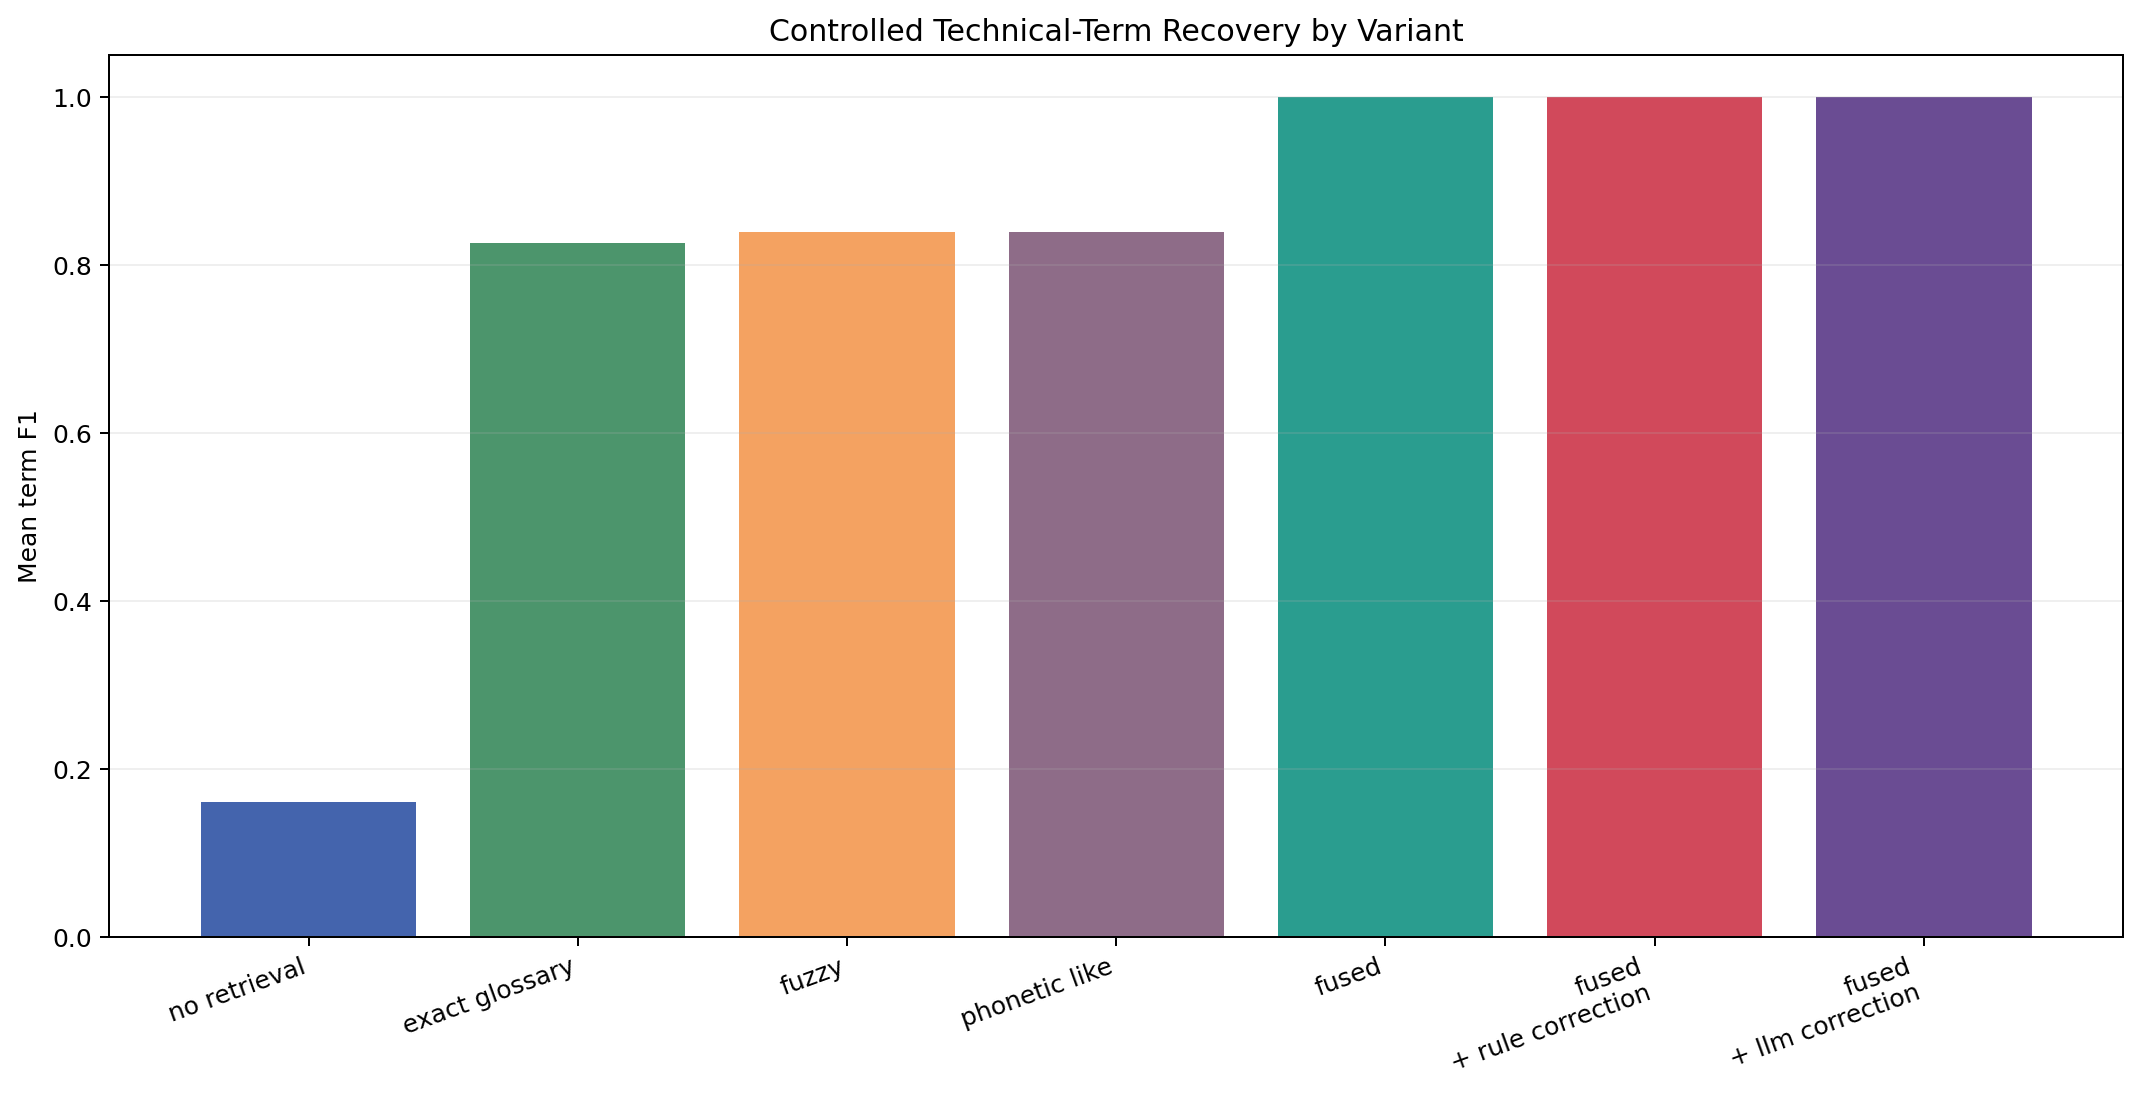
\includegraphics[width=\columnwidth]{figures/term_rescue_f1_by_variant.png}
\caption{Controlled term-rescue F1 by variant. These are text-fixture results; they support mechanism testing only. Exact source paths are listed in the manifest and claim audit.}
\label{fig:app_term_f1}
\end{figure}

\begin{table}[h]
\centering
\scriptsize
\begin{tabular}{llrrrr}
\toprule
Variant & Group & Cases & Term F1 & Error after & Review \\
\midrule
no retrieval & en easy & 7 & 0.000 & 0.218 & 0 \\
fused & en hard & 5 & 1.000 & 0.351 & 0 \\
fused+rule & en hard & 5 & 1.000 & 0.000 & 0 \\
fused+LLM & en hard & 5 & 1.000 & 0.223 & 2 \\
fused+rule & negative control & 4 & 1.000 & 0.000 & 4 \\
\bottomrule
\end{tabular}
\caption{Selected controlled term-rescue rows. The negative-control review count is a safety behavior, not a public-audio performance claim.}
\label{tab:app_term_rows}
\end{table}

\subsection{Controlled Overlap Safety}

\begin{figure}[h]
\centering
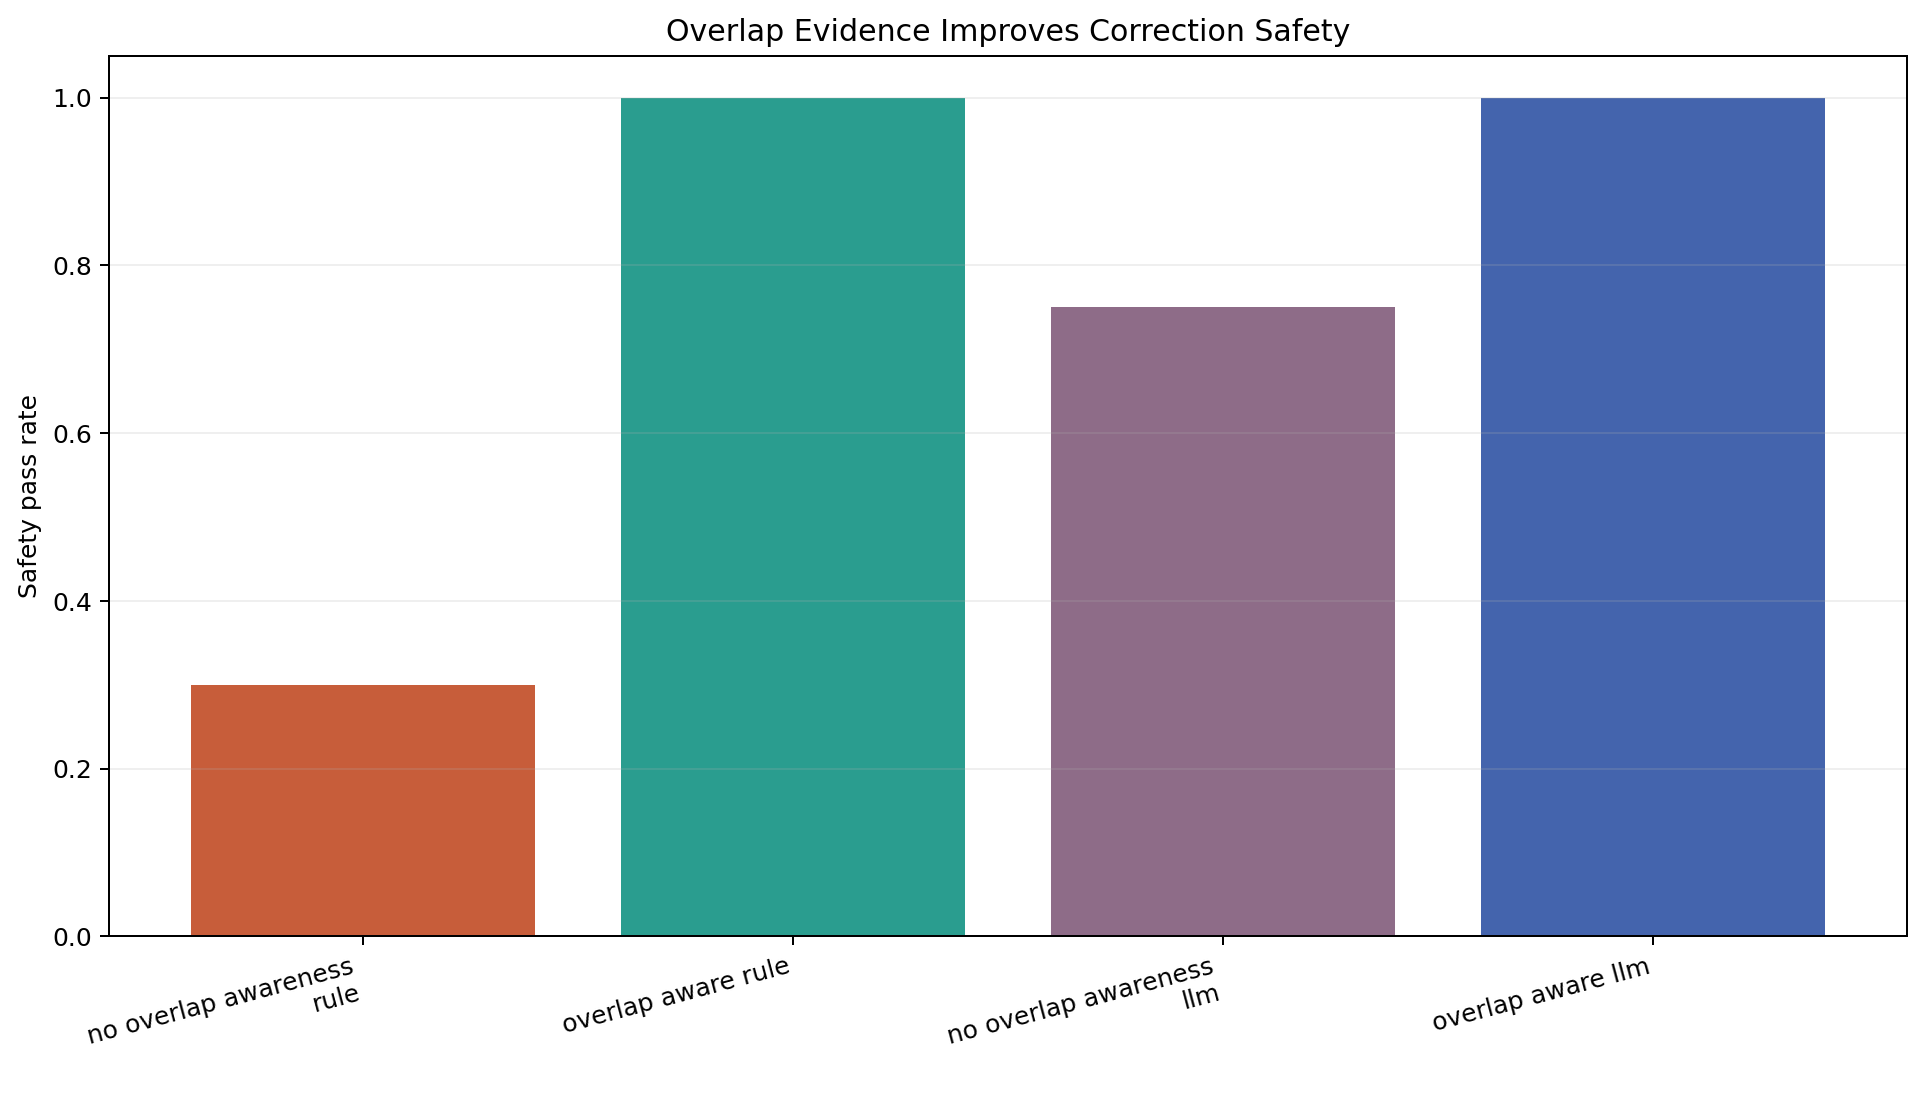
\includegraphics[width=\columnwidth]{figures/overlap_safety_pass_rate.png}
\caption{Controlled overlap safety pass rate generated from the controlled overlap summary.}
\label{fig:app_overlap_safety}
\end{figure}

\begin{table}[h]
\centering
\scriptsize
\begin{tabular}{llrrrr}
\toprule
Variant & True overlap & Uncertainty & Cases & Safety pass & Forbidden \\
\midrule
overlap-aware rule & true & high & 4 & 1.000 & 0 \\
overlap-aware LLM & true & high & 4 & 1.000 & 0 \\
no-overlap rule & true & high & 4 & 0.000 & 3 \\
no-overlap LLM & true & high & 4 & 0.500 & 0 \\
\bottomrule
\end{tabular}
\caption{Selected high-overlap controlled safety rows.}
\label{tab:app_overlap_rows}
\end{table}

\subsection{EvidenceGate Leakage and Held-out Failure}

\begin{figure}[h]
\centering
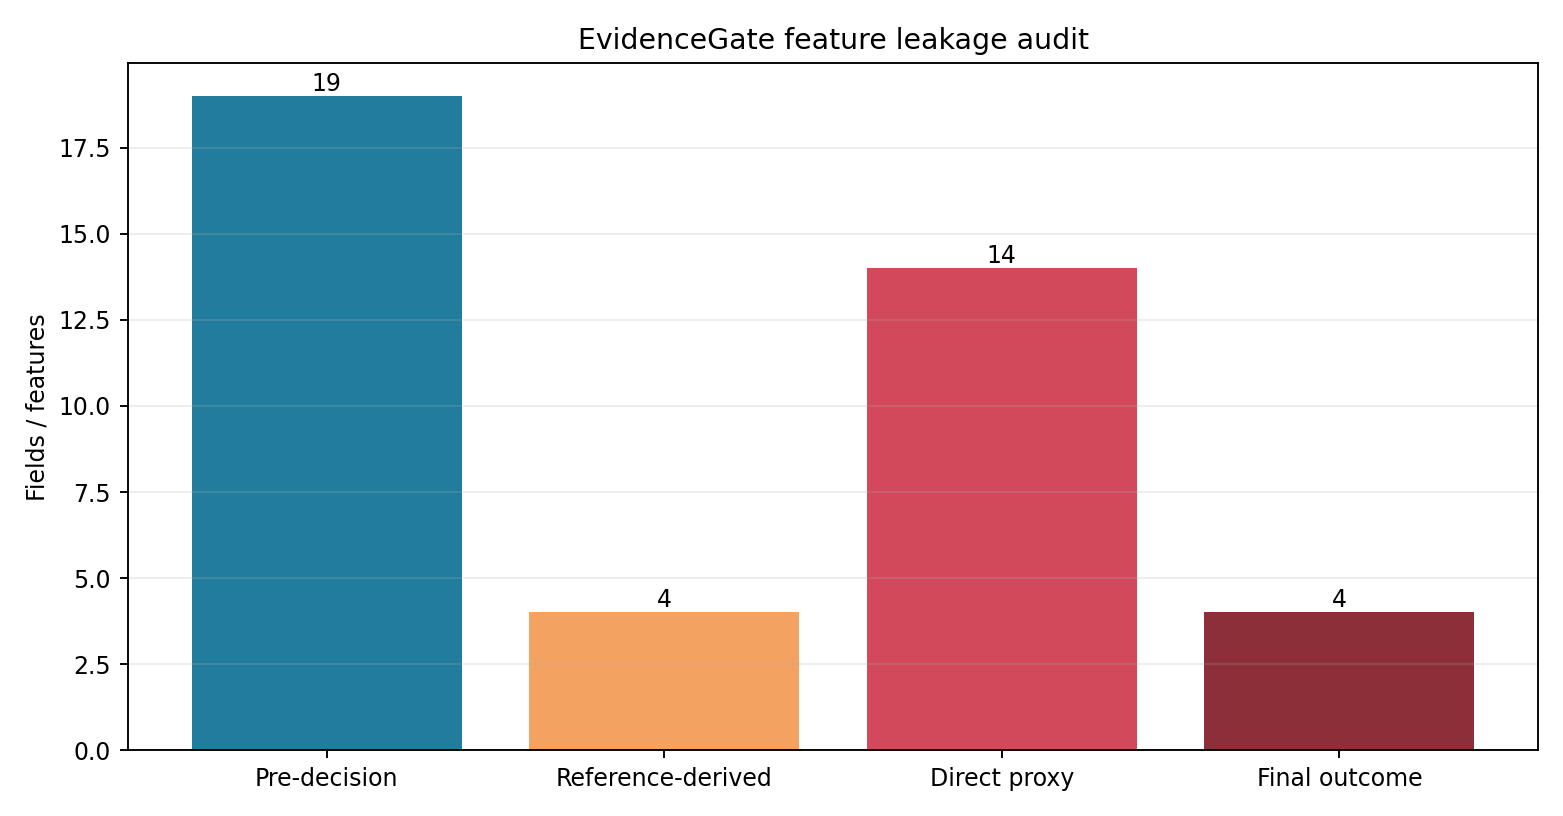
\includegraphics[width=\columnwidth]{figures/evidence_gate_feature_leakage_audit.png}
\caption{EvidenceGate feature leakage audit. The source document reports 41 audited fields: 19 allowed pre-decision, 4 risky reference-derived, 14 direct label proxy, and 4 final audit outcome fields.}
\label{fig:app_evidence_leakage}
\end{figure}

\begin{figure}[h]
\centering
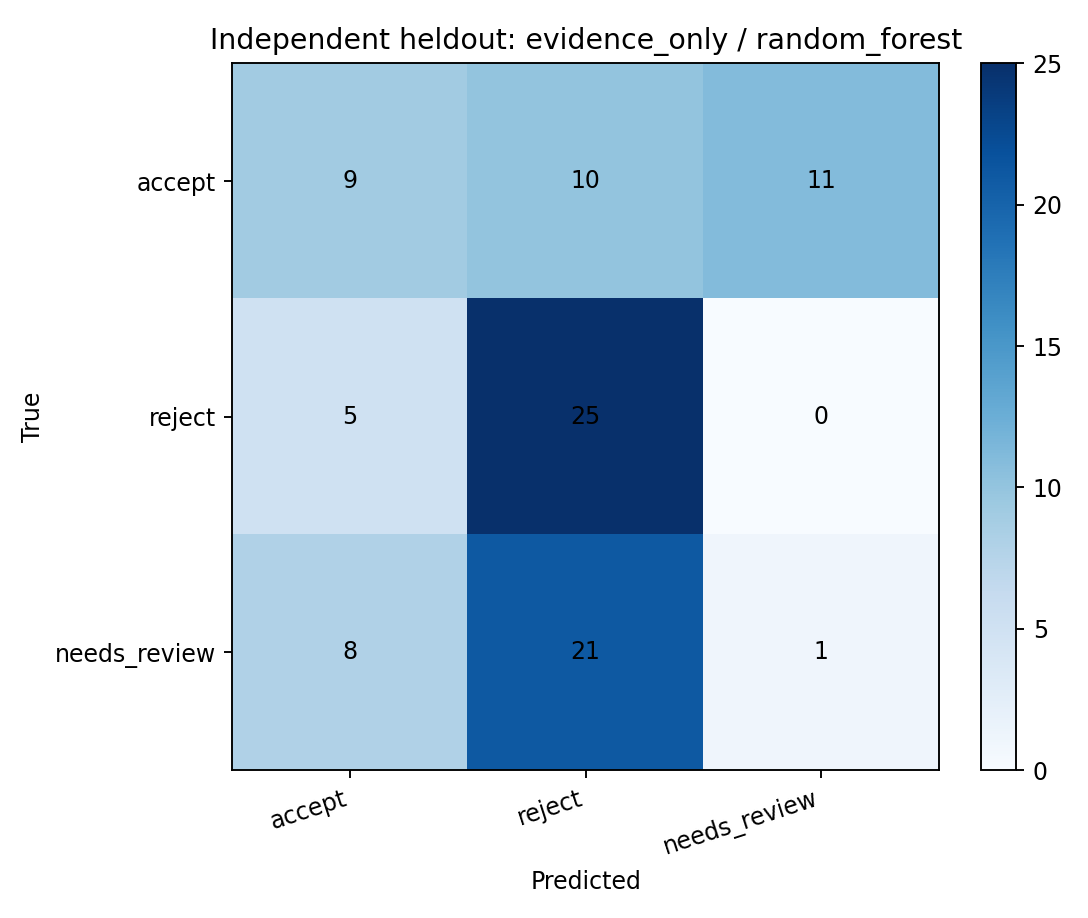
\includegraphics[width=\columnwidth]{figures/evidence_gate_heldout_confusion_matrix.png}
\caption{Independent held-out EvidenceGate confusion matrix. The associated metrics show weak generalization, especially for needs-review routing.}
\label{fig:app_evidence_confusion}
\end{figure}

\begin{table}[h]
\centering
\scriptsize
\begin{tabular}{llrrrr}
\toprule
Feature/model & Split & Macro F1 & False accept & Unsafe accept & Review recall \\
\midrule
audit-aware RF & grouped & 1.000 & 0.000 & 0.000 & 1.000 \\
evidence-only RF & grouped & 0.976 & 0.000 & 0.000 & 0.962 \\
risk-only RF & grouped & 0.924 & 0.133 & 0.000 & 0.769 \\
evidence-only RF & independent & 0.325 & 0.217 & 0.167 & 0.033 \\
evidence-only LR & independent & 0.316 & 0.100 & 0.067 & 0.000 \\
\bottomrule
\end{tabular}
\caption{EvidenceGate validation rows from the EvidenceGate metrics CSV and document. The audit-aware grouped result is a policy-distillation sanity check.}
\label{tab:app_evidence_gate}
\end{table}

\subsection{Binary Safe-to-Apply Stress Test}

\begin{figure}[h]
\centering
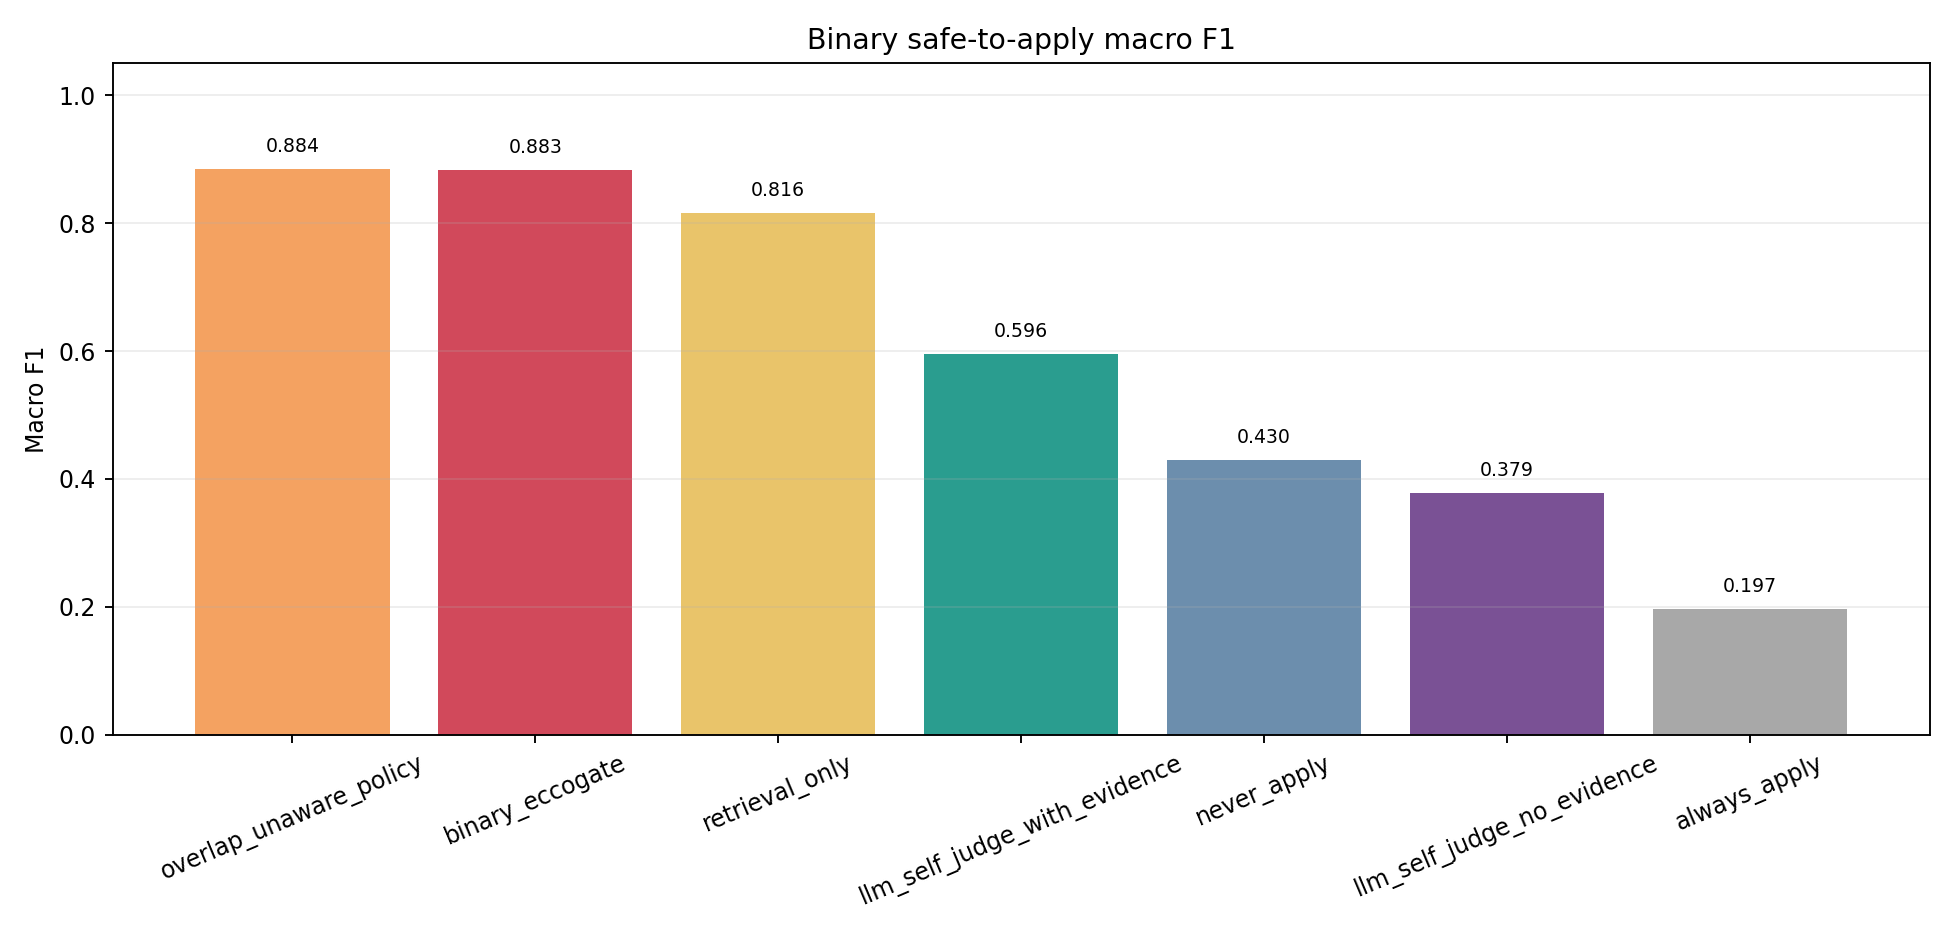
\includegraphics[width=\columnwidth]{figures/binary_safe_apply_macro_f1.png}
\caption{Binary safe-to-apply macro F1. The benchmark is controlled/pilot, not real-audio generalization.}
\label{fig:app_binary_f1}
\end{figure}

\begin{table}[h]
\centering
\scriptsize
\begin{tabular}{lrrrr}
\toprule
Method & Examples & Macro F1 & Unsafe apply & Coverage \\
\midrule
always apply & 327 & 0.197 & 1.000 & 1.000 \\
retrieval only & 327 & 0.816 & 0.198 & 0.385 \\
overlap-unaware policy & 327 & 0.884 & 0.077 & 0.272 \\
binary EccoGate & 327 & 0.883 & 0.053 & 0.239 \\
LLM judge with evidence & 327 & 0.596 & 0.324 & 0.385 \\
\bottomrule
\end{tabular}
\caption{Selected binary safe-to-apply rows.}
\label{tab:app_binary}
\end{table}

\subsection{Interruption Candidate Review}

\begin{table}[h]
\centering
\scriptsize
\begin{tabular}{lrrrrr}
\toprule
Candidates & Reviewed & Interruption & Other labels & Precision & Recall/F1 \\
\midrule
10 & 10 & 10 & 0 & 1.000 & unavailable \\
\bottomrule
\end{tabular}
\caption{Human-reviewed interruption candidate summary. Precision is candidate precision only; recall and F1 are unavailable.}
\label{tab:app_interruption}
\end{table}

\subsection{Runtime and Mobile-Style Evidence}

\begin{figure}[h]
\centering

\includegraphics[width=\columnwidth]{figures/asr_rtf_by_model.png}
\caption{ASR real-time factor chart. This figure supports local runtime trade-off discussion only.}
\label{fig:app_rtf}
\end{figure}

\begin{table}[h]
\centering
\scriptsize
\begin{tabular}{llrrrr}
\toprule
Dataset & Model & Rows & Error & Cleaned error & RTF \\
\midrule
AMI & tiny & 8 & 0.382 & 0.314 & 0.031 \\
AMI & base & 8 & 0.351 & 0.280 & 0.056 \\
FLEURS en & tiny & 10 & 0.186 & 0.186 & 0.072 \\
FLEURS en & base & 10 & 0.134 & 0.134 & 0.140 \\
\bottomrule
\end{tabular}
\caption{Selected local-machine whisper.cpp Level 1 rows. These are not phone-device measurements.}
\label{tab:app_mobile}
\end{table}


\end{document}
